\paragraph{History}
Released in 2004 by Martin Odersky. Provides support for functional programming. Designed to be compiled to Java bytecode, so that Scala applications can be executed on a Java Virtual Machine (JVM).

\paragraph{Basic setup}
Scala has a tool called the REPL (Read-Eval-Print Loop) that is analogous to
  commandline interpreters in many other languages. You may type any Scala
  expression, and the result will be evaluated and printed.

Results are saved as values and may be used in future expressions.

REPL sessions can be saved and loaded using \texttt{:save [path]} and \texttt{:load [path]}.

Recent history can be shown with \texttt{:h?}.

Full programs have the following form. The entry point is defined using an object with a single method, \texttt{main}.
\begin{lstlisting}[language=scala, style=program]
object Application {
  def main(args: Array[String]): Unit = {
    // stuff goes here.
  }
}
\end{lstlisting}

\subparagraph{I/O.} Printing can be done with \texttt{println("Hello world!")}, which forces a newline on next print, or with \texttt{print("Hello world!")}, which does not.

To read a file line by line
\begin{lstlisting}[language=scala, style=snippet]
import scala.io.Source
for(line <- Source.fromFile("myfile.txt").getLines())
  println(line)
\end{lstlisting}

To write a file using Java's \texttt{PrintWriter}
\begin{lstlisting}[language=scala, style=snippet]
val writer = new PrintWriter("myfile.txt")
writer.write("Writing line for line" + util.Properties.lineSeparator)
writer.write("Another line here" + util.Properties.lineSeparator)
writer.close()
\end{lstlisting}

\subparagraph{Importing.}
\begin{lstlisting}[language=scala, style=snippet]
// --- Importing things
import scala.collection.immutable.List
// --- Import all "sub packages"
import scala.collection.immutable._
// --- Import multiple classes in one statement
import scala.collection.immutable.{List, Map}
// --- Rename an import using '=>'
import scala.collection.immutable.{List => ImmutableList}
// --- Import all classes, except some. The following excludes Map and Set:
import scala.collection.immutable.{Map => _, Set => _, _}
// --- Java classes can also be imported. Scala syntax can be used
import java.swing.{JFrame, JWindow}
\end{lstlisting}


\paragraph{Syntactic elements}

Comments:
\begin{lstlisting}[language=scala, style=snippet]
// Single line comment
/*
Multiline
comment
*/
\end{lstlisting}

Scala is strongly typed. Types can be checked without evaluating the expression. (This can be done in the REPL with \texttt{:type}).

\subparagraph{Blocks}
Expressions can be combined by surrounding them with braces \texttt{\{\}}.
\begin{lstlisting}[language=scala, style=snippet]
println(7) // Prints 7

println {
  val i = 5
  i + 2
} // Prints 7
\end{lstlisting}

\paragraph{Values, variables and data types}
Values are like immutable variables, variables are mutable. Declaration is done with the \texttt{val} and \texttt{var} keywords, respectively.
\begin{lstlisting}[language=scala, style=snippet]
val x = 10 // x is now 10
x = 20     // error: reassignment to val
var y = 10
y = 20     // y is now 20
\end{lstlisting}
Even though Scala is a statically typed language, explicit type declaration is often not needed, due to \textit{type inference}. Explicit type declarations can be done as follows:
\begin{lstlisting}[language=scala, style=snippet]
val z: Int = 10
val a: Double = 1.0
val b: Double = 10
\end{lstlisting}

Scala is considered a pure object-oriented language because every value is an object. Hence there are no primitives in Scala (unlike Java which has ,e.g., \texttt{int}s).

There are eight basic types in Scala: \texttt{Byte, Short, Int, Long, Float, Double, Char, Boolean}.

\begin{figure}[h]
\label{scalaTypeHierarchy}
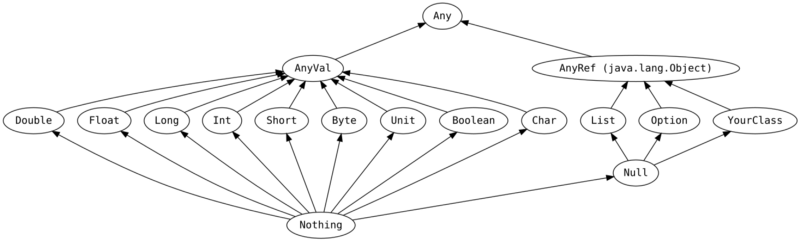
\includegraphics[width=\textwidth]{scalaTypeHierarchy}
\centering
\end{figure}

Every basic Scala type inherits from \texttt{AnyVal}. On the other side, \texttt{AnyRef} is an alias for \texttt{java.lang.Object}. Lastly, both \texttt{AnyVal} and \texttt{AnyRef} inherits from \texttt{Any}.

\subparagraph{Numeric types}:
\begin{lstlisting}[language=scala, style=snippet]
1 + 1   // 2
2 - 1   // 1
5 * 3   // 15
6 / 2   // 3
6 / 4   // 1
6.0 / 4 // 1.5
6 / 4.0 // 1.5
\end{lstlisting}

\subparagraph{Booleans.} Scala supports the Boolean values \texttt{true} an \texttt{false}, as well as the common Boolean operations.
\begin{lstlisting}[language=scala, style=snippet]
!true         // false
!false        // true
true == false // false
10 > 5        // true
\end{lstlisting}

\subparagraph{Strings}
Strings are surrounded by double quotes. Single quotes only used for chars. Triple double-quotes let strings span multiple rows and contain quotes.
\begin{lstlisting}[language=scala, style=snippet]
"Scala strings are surrounded by double quotes"
'a' // A Scala Char
val html = """<form id="daform">
                <p>Press belo', Joe</p>
                <input type="submit">
              </form>"""
\end{lstlisting}
\undline{String interpolation} can be used to embed values directly in string literals.
\begin{lstlisting}[language=scala, style=snippet]
val name = "Bob"
println(s"Hello $name!") // Hello Bob!
\end{lstlisting}
The \texttt{s} before the string is a \udef{string interpolator}. Out of the box Scala provides three string interpolators, but we can create our own as well.
\begin{enumerate}
\item The \textbf{\texttt{s} interpolator} allows variables to be inserted into a string, as shown above. Arbitrary expressions can also be inserted:
\begin{lstlisting}[language=scala, style=snippet]
println(s"1 + 1 = ${1 + 1}")
\end{lstlisting}
\item The \textbf{\texttt{f} interpolator} allows creation of formatted strings. All variable references should be followed by a format string:
\begin{lstlisting}[language=scala, style=snippet]
val height = 1.9d
val name = "James"
println(f"$name%s is $height%2.2f meters tall")  // James is 1.90 meters tall
\end{lstlisting}
Allowed format strings are outlines in the Formatter javadoc: \url{https://docs.oracle.com/javase/6/docs/api/java/util/Formatter.html#detail}
The \texttt{f} interpolator is typesafe. If you try to pass a format string that only works for integers but pass a double, the compiler will issue an error.
\item The \textbf{\texttt{raw} interpolator} is like the \texttt{s} interpolator, except it performs no escaping of literals within the string.
\begin{lstlisting}[language=scala, style=snippet]
scala> raw"a\nb"
res1: String = a\nb
\end{lstlisting}
\end{enumerate}

\subparagraph{Array.} Instantiation using an array literal and accessing elements of an array works as follows (with type inference):
\begin{lstlisting}[language=scala, style=snippet]
val a = Array(1, 2, 3, 5, 8, 13)
a(0)     // Int = 1
a(3)     // Int = 5
a(21)    // Throws an exception
\end{lstlisting}
We can also declare an array as follows
\begin{lstlisting}[language=scala, style=snippet]
val a = new Array[Int](2)
a(0) = 5
a(1) = 2
\end{lstlisting}
Despite being declared as a \texttt{val} in this example, the \texttt{Array} object is mutable so we can change the value of indexes $0$ and $1$. The designation \texttt{val} just means \texttt{a} cannot reference a different array. The array itself may be modified in situ.

A \textbf{\texttt{List}} is like an array, but is immutable.

\subparagraph{Map.} Initialization is as follows:
\begin{lstlisting}[language=scala, style=snippet]
val colours = Map("red" -> "#FF0000", "azure" -> "#F0FFFF", "peru" -> "#CD853F")
colours("red") // java.lang.String = FF0000
\end{lstlisting}
A \texttt{Map} is an immutable data structure. Adding an element means creating another \texttt{Map}.

Maps can have a default value:
\begin{lstlisting}[language=scala, style=snippet]
val safeColours = safeColours.withDefaultValue("Unknown")
safeColours("green")   // java.lang.String = "Unknown"
\end{lstlisting}

Mutable maps exist in \texttt{scala.collection.mutable.Map}.
\begin{lstlisting}[language=scala, style=snippet]
val states = scala.collection.mutable.Map("AL" -> "Alabama", "AK" -> "tobedefined")
states("AK") = "Alaska"
\end{lstlisting}

\subparagraph{Sets} are Iterables that contain no duplicate elements. We test for set membership with parentheses.
\begin{lstlisting}[language=scala, style=snippet]
val s = Set(1, 3, 7)
s(0)      // Boolean = false
s(1)      // Boolean = true
\end{lstlisting}

\subparagraph{Tuples} are immutable and contain a fixed number of elements, each with a distinct type. Literals use parentheses.
\begin{lstlisting}[language=scala, style=snippet]
val d = (3, 1, "five")
(colours, states)
\end{lstlisting}
Accessing elements of tuples is done with \texttt{.\_n}, where \texttt{n} is the 1-based index of the element.
\begin{lstlisting}[language=scala, style=snippet]
d._1    // Int = 3
d._2    // Int = 1
\end{lstlisting}
Tuples can also be unpacked:
\begin{lstlisting}[language=scala, style=snippet]
val (div, mod) = divideInts(10, 3)
div     // Int = 3
mod     // Int = 1
\end{lstlisting}

\paragraph{Flow control}
\begin{itemize}
\item \textbf{If-else}
\begin{lstlisting}[language=scala, style=snippet]
if (condition1) {

} else if (condition2) {

} else {

}
\end{lstlisting}
It is also an expression.
\begin{lstlisting}[language=scala, style=snippet]
def max(x: Int, y: Int) = if (x > y) x else y
\end{lstlisting}
\item Basic for loop:
\begin{lstlisting}[language=scala, style=snippet]
// a goes from 0 to 10 inclusive
for (a <- 0 to 10) {
  println(a)
}
// a goes from 0 to 10 exclusive
for (a <- 0 until 10) {
  println(a)
}
// Looping over two elements
for (a <- 0 until 2; b <- 0 to 2) {
  println((a,b))
}
\end{lstlisting}
\item Looping over iterable (with optional condition):
\begin{lstlisting}[language=scala, style=snippet]
for (elem <- list if elem % 2 == 0) {
  
}
\end{lstlisting}
\item For comprehension functions as a generator
\begin{lstlisting}[language=scala, style=snippet]
val sub = for (elem <- list if elem % 2 == 0) yield elem
\end{lstlisting}
\end{itemize}
Exceptions can be handled in two ways.
\begin{lstlisting}[language=scala, style=snippet]
try {
  val n = new FileReader("input.txt").read()
  println(s"Success: $n")
} catch {
  case e: Exception =>
    e.printStackTrace
}
\end{lstlisting}
Or using \texttt{Try}.
\begin{lstlisting}[language=scala, style=snippet]
val tried: Try[Int] = Try(new FileReader("notes.md")).map(f => f.read())
    
tried match {
  case Success(n) => println(s"Success: $n")
  case Failure(e) => e.printStackTrace
}
\end{lstlisting}

\paragraph{Methods.}
A method is a function that is a member of a class, trait or object.
A basic method example:
\begin{lstlisting}[language=scala, style=snippet]
def add(x: Int, y: Int): Int = {
  x + y
}
\end{lstlisting}
Parameters are immutable. The \texttt{return} keyword is optional. The method will automatically return the last expression. \texttt{return} exits the current method, not the current block (as opposed to Java).
 
The return type is optional. The Scala compiler is also able to infer it.

Methods without output can be written two ways
\begin{lstlisting}[language=scala, style=snippet]
def printSomething(s: String) = {
  println(s)
}
def printSomething(s: String): Unit = {
  println(s)
}
\end{lstlisting}
Multiple outputs can be returned using tuples.
\begin{lstlisting}[language=scala, style=snippet]
def increment(x: Int, y: Int): (Int, Int) = {
  (x + 1, y + 1)
}
\end{lstlisting}
A method without arguments can be called without parentheses. Best practice dictates that this syntax is to be used if the method does not have any side-effects. (See also the \texttt{Dog} class below).

The last parameter can be allowed to take any number of arguments, using an asterisk
\begin{lstlisting}[language=scala, style=snippet]
def variablesArguments(args: Int*): Int = {
  var n = 0
  for (arg <- args) {
    n += arg
  }
  n
}
\end{lstlisting}
We can also give parameters default values. The default parameter may be used by providing \texttt{\_} as an argument (or using named arguments).
\begin{lstlisting}[language=scala, style=snippet]
def default(x: Int = 1, y: Int): Int = {
  x * y
}
default(_, 3)  // Int = 3
default(y = 3) // Int = 3
\end{lstlisting}

Methods may also be nested inside other methods.

\paragraph{Functions.}
Functions are first-class in Scala. This means methods can take a function as a parameter.
\begin{lstlisting}[language=scala, style=snippet]
def foo(i: Int, f: Int => Int): Int = {
  f(i)
}
\end{lstlisting}
Function literals defined as follows
\begin{lstlisting}[language=scala, style=snippet]
val increment: Int => Int = (x: Int) => x + 1
val divideInts: (Int, Int) => (Int, Int) = (x: Int, y: Int) => (x / y, x % y)
\\ Or, using type inference:
val divideInts = (x: Int, y: Int) => (x / y, x % y)
\end{lstlisting}
By not assigning a function to a variable, we get an anonymous function.

Scala supports closures.

Partial functions can be implemented with the following syntax
\begin{lstlisting}[language=scala, style=snippet]
def speed(distance: Float, time: Float): Float = {
  distance / time
}
val partialSpeed: Float => Float = speed(5, _)
\end{lstlisting}

\paragraph{Classes, objects and traits}
\subparagraph{Classes} Example of a class:
\begin{lstlisting}[language=scala, style=snippet]
class Dog(br: String) {
  var breed: String = br
  def bark = "Woof, woof!"

  private def sleep(hours: Int) =
    println(s"I'm sleeping for $hours hours")
}

val mydog = new Dog("greyhound")
println(mydog.breed) // => "greyhound"
println(mydog.bark) // => "Woof, woof!"
\end{lstlisting}
Values and methods are assumed public. Values declared with \texttt{val} cannot be changed. \texttt{protected} (members are only accessible from sub-classes) and \texttt{private} (members are only accessible from the current class/object) keywords are also available. We can also make a method private only outside a package.

Scala supports two types of constructors:
\begin{enumerate}
\item The \textbf{primary constructor} is anything defined in the body of the class except method declarations. The parameter list comes after the class name and may contain default values. It may be omitted. Only a primary constructor is allowed to invoke a superclass constructor. A primary constructor may be made private by using the \texttt{private} keyword between the class name and the constructor parameter-list.
\item \textbf{Auxiliary contructors} are like methods with the name \texttt{this}. They must call a previously defined constructor, i.e. a primary or auxiliary constructor that lexically precedes it. The first statement of the auxiliary constructor must contain the constructor call using \texttt{this}.
\begin{lstlisting}[language=scala, style=snippet]
class GFG( Aname: String, Cname: String) 
{ 
    var no: Int = 0;; 
    def display() 
    { 
        println("Author name: " + Aname); 
        println("Chapter name: " + Cname); 
        println("Total number of articles: " + no); 
          
    } 
      
    // Auxiliary Constructor 
    def this(Aname: String, Cname: String, no:Int)  
    { 
        // Invoking primary constructor 
        this(Aname, Cname) 
        this.no=no 
    } 
} 
\end{lstlisting}
\end{enumerate}

Abstract methods are methods with no body. A class with abstract methods must be declared \texttt{abstract}.
\begin{lstlisting}[language=scala, style=snippet]
abstract class Dog(br: String) {
  var breed: String = br
  def chaseAfter(what: String): String
}
\end{lstlisting}

\subparagraph{Objects} The \texttt{object} keyword creates a type and a singleton instance of it. Objects and classes can have the same name.
\begin{lstlisting}[language=scala, style=snippet]
object Dog {
  def allKnownBreeds = List("pitbull", "shepherd", "retriever")
  def createDog(breed: String) = new Dog(breed)
}
\end{lstlisting}

\subparagraph{Case classes} Case classes are like classes, but are primarily used to create data containers. They are immutable. Classes proper tend to focus on objects oriented concept, such as encapsulation, polymorphism, and behavior. The values tend to be private and only the methods exposed.

\begin{lstlisting}[language=scala, style=snippet]
case class Person(name: String, phoneNumber: String)

val george = Person("George", "1234")
val kate = Person("Kate", "4567")
\end{lstlisting}
Cases classes don't need \texttt{new}.

Case classes have extra functionality built in, such as
\begin{itemize}
\item getters
\begin{lstlisting}[language=scala, style=snippet]
george.phoneNumber  // => "1234"
\end{lstlisting}
\item per field equality (no need to override .equals)
\begin{lstlisting}[language=scala, style=snippet]
Person("George", "1234") == Person("Kate", "1236")  // => false
\end{lstlisting}
\item easy way to copy
\begin{lstlisting}[language=scala, style=snippet]
val otherGeorge = george.copy(phoneNumber = "9876")
\end{lstlisting}
\end{itemize}

\subparagraph{Traits}
Similar to Java interfaces, traits define an object type and method signatures. Scala allows partial implementation of those methods. Constructor parameters are not allowed. Traits can inherit from other traits or classes without parameters. A trait method can also have a default implementation.
\begin{lstlisting}[language=scala, style=snippet]
trait Dog {
    def breed: String
    def color: String
    def bark: Boolean = true
    def bite: Boolean
}
class SaintBernard extends Dog {
    val breed = "Saint Bernard"
    val color = "brown"
    def bite = false
}
\end{lstlisting}
A trait can also be used as a mixin. The class ``extends'' the first trait, but the keyword \texttt{with} can add additional traits.
\begin{lstlisting}[language=scala, style=snippet]
trait Bark {
    def bark: String = "Woof"
}
trait Dog {
    def breed: String
    def color: String
}
class SaintBernard extends Dog with Bark {
    val breed = "Saint Bernard"
    val color = "brown"
}
\end{lstlisting}

\paragraph{Generics}
TODO

\paragraph{Pattern matching}
Like a switch statement, but much more powerful.
\begin{lstlisting}[language=scala, style=snippet]
def matchEverything(obj: Any): String = obj match {
  // You can match values:
  case "Hello world" => "Got the string Hello world"

  // You can match by type:
  case x: Double => "Got a Double: " + x

  // You can specify conditions:
  case x: Int if x > 10000 => "Got a pretty big number!"

  // You can match case classes as before:
  case Person(name, number) => s"Got contact info for $name!"

  // You can match regular expressions:
  case email(name, domain) => s"Got email address $name@$domain"

  // You can match tuples:
  case (a: Int, b: Double, c: String) => s"Got a tuple: $a, $b, $c"

  // You can match data structures:
  case List(1, b, c) => s"Got a list with three elements and starts with 1: 1, $b, $c"

  // You can nest patterns:
  case List(List((1, 2, "YAY"))) => "Got a list of list of tuple"

  // Match any case (default) if all previous haven't matched
  case _ => "Got unknown object"
}
\end{lstlisting}

\paragraph{Currying and implicits} TODO

\paragraph{Concurrency}
TODO